%======================================================
% This file is part of
% "AMCOS_booklet"
% Version 1.1 (04/07/2019)
% A LaTeX template for conference books of abstracts
%
% This template is available at:
% https://github.com/maximelucas/AMCOS_booklet
%
% License: GNU General Public License v3.0
%
% Authors:
% Maxime Lucas (ml.maximelucas@gmail.com)
% Pau Clusella
%=======================================================

\documentclass[openany, parskip=full, 12pt, a4]{scrbook}
\usepackage{etoolbox,auxhook}
\usepackage{rotating}

%======================================================
% This file is part of
% "AMCOS_booklet"
% Version 1.1 (04/07/2019)
% A LaTeX template for conference books of abstracts
%
% This template is available at:
% https://github.com/maximelucas/AMCOS_booklet
%
% License: GNU General Public License v3.0
%
% Authors:
% Maxime Lucas (ml.maximelucas@gmail.com)
% Pau Clusella
%=======================================================

\usepackage[utf8]{inputenc}
\usepackage[T1]{fontenc}

%---------------------------------------------------------
% PACKAGES
%---------------------------------------------------------

% TYPOGRAPHY
\usepackage{xspace}
\usepackage{microtype}
\usepackage{cmbright} % different fonts

% VARIA
\usepackage{color}
\usepackage[table]{xcolor} % loads also »colortbl« %load before tikz if options
\usepackage{scrhack} % fix koma script warning about addtolist
\usepackage{blindtext}
\usepackage{pdfpages} % for cover 

\usepackage{ifthen} % to have online and printed versionw

% GRAPHICS & FIGURES & TABLES
\usepackage{graphicx}
\usepackage{float}
\usepackage{multicol} % for timetable
\usepackage{longtable} % for list of participants over more than 1 page
%\usepackage{wrapfig}
%\usepackage{tikz}
%\tikzset{ar/.style={>=latex, ->}}
%\renewcommand{\arraystretch}{1.2}
%\usepackage[multidot]{grffile}
% \usepackage{booktabs}

% WANTS TO BE LAST
\usepackage[english]{babel}

\usepackage[hidelinks]{hyperref}
\hypersetup{pdfpagelayout=TwoPageRight}
% \usepackage[ocgcolorlinks]{hyperref}
% \hypersetup{colorlinks, linkcolor={wolf}, linktocpage=true, citecolor ={tpred}, urlcolor={black}}


%-------------------------------------------------------------
% SETTINGS
%-------------------------------------------------------------
\pagestyle{plain}

\setcounter{secnumdepth}{-2} % remove numbering at any level both for the heading and the toc
%https://tex.stackexchange.com/questions/30122/generate-table-of-contents-when-section-sections-without-numbering-has-been

%-------------------------------------------------------------
% USEFUL DEFINTIONS
%-------------------------------------------------------------

% VARIA 
\newcommand\tab[1][1cm]{\hspace*{#1}}


%======================================================
% This file is part of
% "AMCOS_booklet"
% Version 1.1 (04/07/2019)
% A LaTeX template for conference books of abstracts
%
% This template is available at:
% https://github.com/maximelucas/AMCOS_booklet
%
% License: GNU General Public License v3.0
%
% Authors:
% Maxime Lucas (ml.maximelucas@gmail.com)
% Pau Clusella
%=======================================================

%
% COLORS
%

\definecolor{myorange}{RGB}{255,184,28}	% SLU orange
\definecolor{mygray}{RGB}{136,139,141 }		% SLU grey
\definecolor{mywhite}{RGB}{235, 238, 231}
\definecolor{myblue}{RGB}{0,102,79}		% SLU green
\definecolor{myred}{RGB}{111,38,61}		% SLU red
\definecolor{mygreen}{RGB}{196,214,0 }		% SLU green äpple
\definecolor{myyellow}{RGB}{252,227,0 }		% SLU green majs

\newcommand{\primarycolor}{myblue}
\newcommand{\secondarycolor}{myred}
\newcommand{\ternarycolor}{mywhite}

%
% BOOKLET VERSIONS
%

% If compilation is done with 'compile.sh', both versions (online and printed) are automatically compiled
% If compilation is done from editor, choose which version to compile below
\makeatletter
\@ifundefined{ifOnline}{% % check if already defined from the command line, if not define \ifOnline
	\expandafter\newif\csname ifOnline\endcsname
	\Onlinefalse %set to \Onlinefalse/\Onlinetrue for printed/online version
}{}
\makeatother

% define \type to input the right version of the abstracts
\ifOnline
\newcommand{\type}{o}
\else
\newcommand{\type}{p}
\fi % end if

%
% ABSTRACT ENVIRONMENTS
%

%----------------------------------------
% online abstract environment
%----------------------------------------
\newenvironment{abstract_online}[4] %{title}{author}{affiliation}{type}
{\filbreak %avoid page break
	
	{\large \bfseries #1}
	
	{\bfseries \itshape #2} \hfill {#3}
	
	\textcolor{mygray}{#4}
	
}
{}

%----------------------------------------
% talk abstract environment (printed)
%----------------------------------------
\newenvironment{abstract}[4] %{title}{author}{affiliation}
{\filbreak %avoid page break
	
	{\large \bfseries #1}
	
	{\bfseries \itshape #2,} \textcolor{mygray}{#3} \hfill {#4}
	
	
}
{}

%----------------------------------------
% poster abstract environment (printed)
%----------------------------------------
\newcommand{\poster}[3] %{title}{author}{affiliation}
{\filbreak %avoid page break
	
	{\bfseries \large #1} \\	
	\tab #2, \textit{#3}
	
}
{}

%----------------------------------------
% tags for talk type (colored circle in abstracts)
%----------------------------------------

\newcommand{\KLtag}{\tikz[baseline={([yshift=-.8ex]current bounding box.center)}]  \node[circle, inner sep=2pt, minimum size=0.5em, color=black, fill=\KLcolor]{\small \bfseries KL};} %colored circle with tag

\newcommand{\IStag}{\tikz[baseline={([yshift=-.8ex]current bounding box.center)}]  \node[circle, inner sep=2pt, minimum size=0.5em, color=black, fill=\IScolor]{\small \bfseries IS};} %colored circle with tag

\newcommand{\CTtag}{\tikz[baseline={([yshift=-.8ex]current bounding box.center)}]  \node[circle, inner sep=2pt, minimum size=0.5em, color=black, fill=\CTcolor]{\small \bfseries CT};} %colored circle with tag

\newcommand{\ITtag}{\tikz[baseline={([yshift=-.8ex]current bounding box.center)}]  \node[circle, inner sep=2pt, minimum size=0.5em, color=black, fill=\ITcolor]{\small \bfseries IT};} %colored circle with tag

%
% PAGE LAYOUT DEFINITIONS
%
\usepackage{etoolbox}

%------------------------------------------------------
% page style: vertical line on the side of each page
%------------------------------------------------------
\usepackage[scale=1,angle=0,opacity=1]{background}
\backgroundsetup{contents={}}

\AddEverypageHook{%
\ifthenelse{%
	\isodd{\thepage} \AND  \thepage>1 % if odd page but not front page
	}{%
	\backgroundsetup{
		color=\secondarycolor,
		position=current page.south east,%
		nodeanchor=south east,
		contents={\rule{10pt}{0.66\paperheight}}
		}
	}{%
	% nothing
	}
%
\ifthenelse{% 
	\NOT \isodd{\thepage} \AND \NOT \thepage=44% if even page
	}{%
	\backgroundsetup{
		color=\secondarycolor,
		position=current page.south west,%
		nodeanchor=south west,
		contents={\rule{10pt}{0.66\paperheight}}
		}
	}{%
	% nothing
	}
\BgMaterial}


%---------------------------------------------------
% chapter heading style
%---------------------------------------------------

\newdimen\mybarpadding
\mybarpadding=1.5em\relax %padding between gcolored bar and chapter name

\RedeclareSectionCommand[%
    ,afterskip=4em plus 1pt minus 1pt%
    ,beforeskip=-1pt%1.2em plus 1pt minus 1pt%
    ,level=0%
    ,toclevel=0%
]{chapter}%

\setkomafont{chapter}{\normalfont\normalsize\bfseries\Huge} % koma-script-specific command

\newcommand*{\mynumberedtest}[1]{% to test whether there is a number
  \if\relax\detokenize{#1}\relax%
  \else%
    #1%
    
  \fi}

%-------------------------------------------------chapter style definition

\renewcommand{\chapterlinesformat}[3]{%
  \ifthispageodd{%
    \hfill%
    \raisebox{-0.2em}{%
      \makebox[0pt][r]{\textcolor{\primarycolor}{\rule{\paperwidth}{1em}}}%
    }%
    \hspace{\mybarpadding}%
% 	\mynumberedtest{#2}
	\mbox{#3}%
  }{%
%    \hbox{%
%       \mynumberedtest{#2}
      \mbox{#3}%
      \hspace{\mybarpadding}%
      \raisebox{-0.2em}{%
        \makebox[0pt][l]{\textcolor{\primarycolor}{\rule{\paperwidth}{1em}}}%
      }%
%    }%
  }%
}
\makeatother
%---------------------------------------------------------

% TIMETABLE COLORS AND STYLES

% text and backgroud colors
\newcommand{\tbg}{gray} % background
\newcommand{\tfg}{white}
\newcommand{\tbc}{gray!25}

% talk types colors
\newcommand{\IScolor}{mygreen} % invited speaker
\newcommand{\CTcolor}{white} % contributed talk


% row types
\newcommand{\tablebreak}[2]{% {time span}{break name}
	\rowcolor{myyellow} #1 &  \multicolumn{3}{c|}{\bfseries #2} \\ \hline }
\newcommand{\eventtype}[2]{% {time span}{event name}
	#1& \multicolumn{3}{c|}{\cellcolor{\tbg}\color{\tfg}\bfseries #2} \\ \hline }

% column spacing and position
\newcolumntype{L}[1]{%
	>{\raggedright\let\newline\\\arraybackslash\hspace{0pt}}m{#1}}
\newcolumntype{C}[1]{%
	>{\centering\let\newline\\\arraybackslash\hspace{0pt}}m{#1}}
\newcolumntype{R}[1]{%
	>{\raggedleft\let\newline\\\arraybackslash\hspace{0pt}}m{#1}}

%\newcommand{\mytable}{|C{0.15\linewidth}| C{0.05\linewidth}|  C{0.25\linewidth} C{0.1\linewidth} C{0.5\linewidth}|}

\newcommand{\IS}[5]{% {time span}{name}{University}{City, Country}{title}
	#1 &\cellcolor{\IScolor}IS&{\bfseries#2}\newline #4&&#5 \\ \hline}
\newcommand{\CT}[4]{%
	#1 & &{\bfseries#2}&#4 \\ \hline}

	
\begin{document}

% COVER PAGE
%--------------------------------------------------------------------

\includepdf{Cover_SLU}	% our cover was produced with canva.com
	
	
% BLANK PAGE
%---------------------------------------------------------------------
\mbox{}
\thispagestyle{empty}
\vfill
\begin{center}
	\ifOnline
\textcolor{white}{slubi}
	\else
\textcolor{white}{slubi}
	\fi % end if
	\\[20pt] % Please cite us by keeping the following line.
	The open-source \LaTeX{} template used to generate this booklet is available at \url{https://github.com/maximelucas/AMCOS\_booklet}
\end{center}

\newpage

% TABLE OF CONTENTS 
%---------------------------------------------------------------------
\tableofcontents

% ABOUT
%---------------------------------------------------------------------
\chapter{About}

{\small \textcolor{myblue}{Welcome to SLU's Day of Bioinformatics! Today we want to present you a range of exciting research, performed at SLU, enabled by bioinformatics. Sit back and enjoy!}}

\section{SLU's Day of Bioinformatics}
This symposium aims to bring together researchers, bioinformaticians and people interested in advances of agricultural sciences from all over SLU (and other places). 


\section{SLUBI}

Today's symposium is organized by SLUBI, SLU's Bioinformatics Infrastructure. SLUBI provides bioinformatics and data science support to SLU's researchers since 2017. We provide a wide spectrum of services, including hands-on assistance for bioinformatics analyses, basic and advanced training and consultation services. 

SLUBI is working in collaboration with NBIS (National Bioinformatics Infrastructure Sweden), SLU's Center for Statistics, as well as SLU's Data Management Center. 


\section{Organizers}
\begin{center}
\begin{tabular}{lcl}
 & \textbf{SLUBI} &  \\
 Amrei Binzer-Panchal & Nicolas Delhomme &  Lizel Potgieter \\
Adnan Niazi &  Iryna Shutava&  Abu Bakar Siddique\\
 &  &  \\
 & \textbf{Section for Bioinformatics} &  \\
Erik Bongcam Rudloff &  Renaud vanDamme &  Samuel Flores \\
\end{tabular}
\end{center}

% TIMETABLE 
%---------------------------------------------------------------------
\chapter{Timetable}

%CT: Contributed Talk, IS: Invited Speaker, KL: Keynote Lecture, IT: Invited Talk.
% Custom commands used here can be found at the end of the preamble_booklet.tex file

\section{Monday, 4th of November}
\begin{center}
	\filbreak
\begin{longtable}{|C{0.15\linewidth}| C{0.0\linewidth}  C{0.3\linewidth} C{0.5\linewidth}|}\hline	
	\tablebreak{9:00--9:15}{Welcome}
	\CT{9:15--09:30}{Gabriella Lindgren}{}{An endothelial regulatory module links blood pressure regulation with elite athletic performance}
	\CT{09:30--09:45}{G\"oran Andersson}{}{Bioinformatics analyses of genomics, epigenomics and transcriptomics data of complex diseases }
	\CT{09:45--10:00}{Jan Ingemar Ohlsson}{}{Bioinformatics R-ABCD: Research Acceleration with Big Cow Data in Gigacow}
	\CT{10:00--10:15}{Michael Landi}{}{Crop diversity and health: assembling the cassava genome }
	\tablebreak{10:15--10:45}{Coffee}
	\CT{10:45--11:30}{\'{A}lvaro Mart\'{i}nez Barrio}{}{20 years of computational biology: where the road has taken us and the highway is leading}
	\CT{11:30--11:45}{Olga Vinnere Pettersson}{}{Latest methods and their applications for agricultural research }
	\CT{11:45--12:00}{Girma Gebresenbet}{}{Digitalization in agricultural practices}
	\tablebreak{12:00--13:00}{Lunch}
	\CT{13:00--13:30}{Discussion}{}{Bioinformatics in Agricultural Sciences, what is here, what is needed?}
	\CT{13:30--13:45}{Sara Hallin}{}{Microbes driving nitrogen losses and retention in soils}
	\CT{13:45--14:00}{Shrikant Sharma}{}{Genome editing in potatoes}
	\tablebreak{14:00--14:15}{Break}
	\CT{14:15--14:30}{Salme Timmusk}{}{Plant-root microbiome interactions}
	\CT{14:30--14:45}{Moritz Buck}{}{Microbial diversity and nutrient cycling in the central arctic ocean}
	\CT{14:45--15:00}{Anna Sz\'ekely}{}{Environmental virus sequencing and genotyping as a tool of epidemiological monitoring}
	\tablebreak{15:00--15:05}{Concluding remarks}
	\eventtype{15:05--16:00}{Open fika and mingling}
\end{longtable}
\end{center}


\section{Tuesday, 5th of November}



% TALKS 
%---------------------------------------------------------------------
%\chapter{List of Abstracts -- Talks}


% Definitions of custom environment used here can be found in preamble_booklet.tex file

% The following input commands automatically select the right version 
% (print or online) version of the abstract's .tex
% \type is defined in preamble_booklet.tex and equals:
% 'o' (online) or 'p' (print)

%\input{abstracts/tex/t\type_tremblay}


% POSTERS
%------------------------------------------------------------------
%\chapter{List of Posters} 

%\vspace{-2.5em}

% \section{Tuesday Session}

%\input{abstracts/tex/p\type_doe}



% LIST OF PARTICIPANTS
%------------------------------------------------------------------
%\chapter{List of Participants}
 
%\input{list_of_participants}
 
% USEFUL INFO
%------------------------------------------------------------------
\chapter{Useful Information}

\begin{center}
\includegraphics[width=\linewidth]{images/VHC.jpg}
\end{center}

\textbf{Talks} will be held at the \textbf{Room S\"arimner} of VHC, \textbf{campus Ultuna}. It is situated on the ground floor and
has access from main entrance of VHC. Please check the following pages for a floor plan of the building. \

Joint \textbf{remote participation} is organized at \textbf{campus Alnarp}, in room \textbf{Triticum}. The room is opposite the blue kitchen in building Horticum, Sundsvägen 10. Please check the following pages for an overview over campus Alnarp. \

Alternatively, individual remote participation is possible via \textbf{Zoom}. A link is send to everyone who signs up to the event. If you haven't received the link, please contact us via amrei.binzer.panchal@slu.se. 
 
\section{How to get to VHC in Ultuna?}

 \textbf{VHC visitor entrance:}\
Ulls väg 26; Ultuna, Uppsala \
GPS: N 59°48'53, E 17°39'30


 \textbf{Bus:} \
 line 4 from central Uppsala, stop Campus Ultuna, VHC is the round building by the bus stop. 


\begin{center}
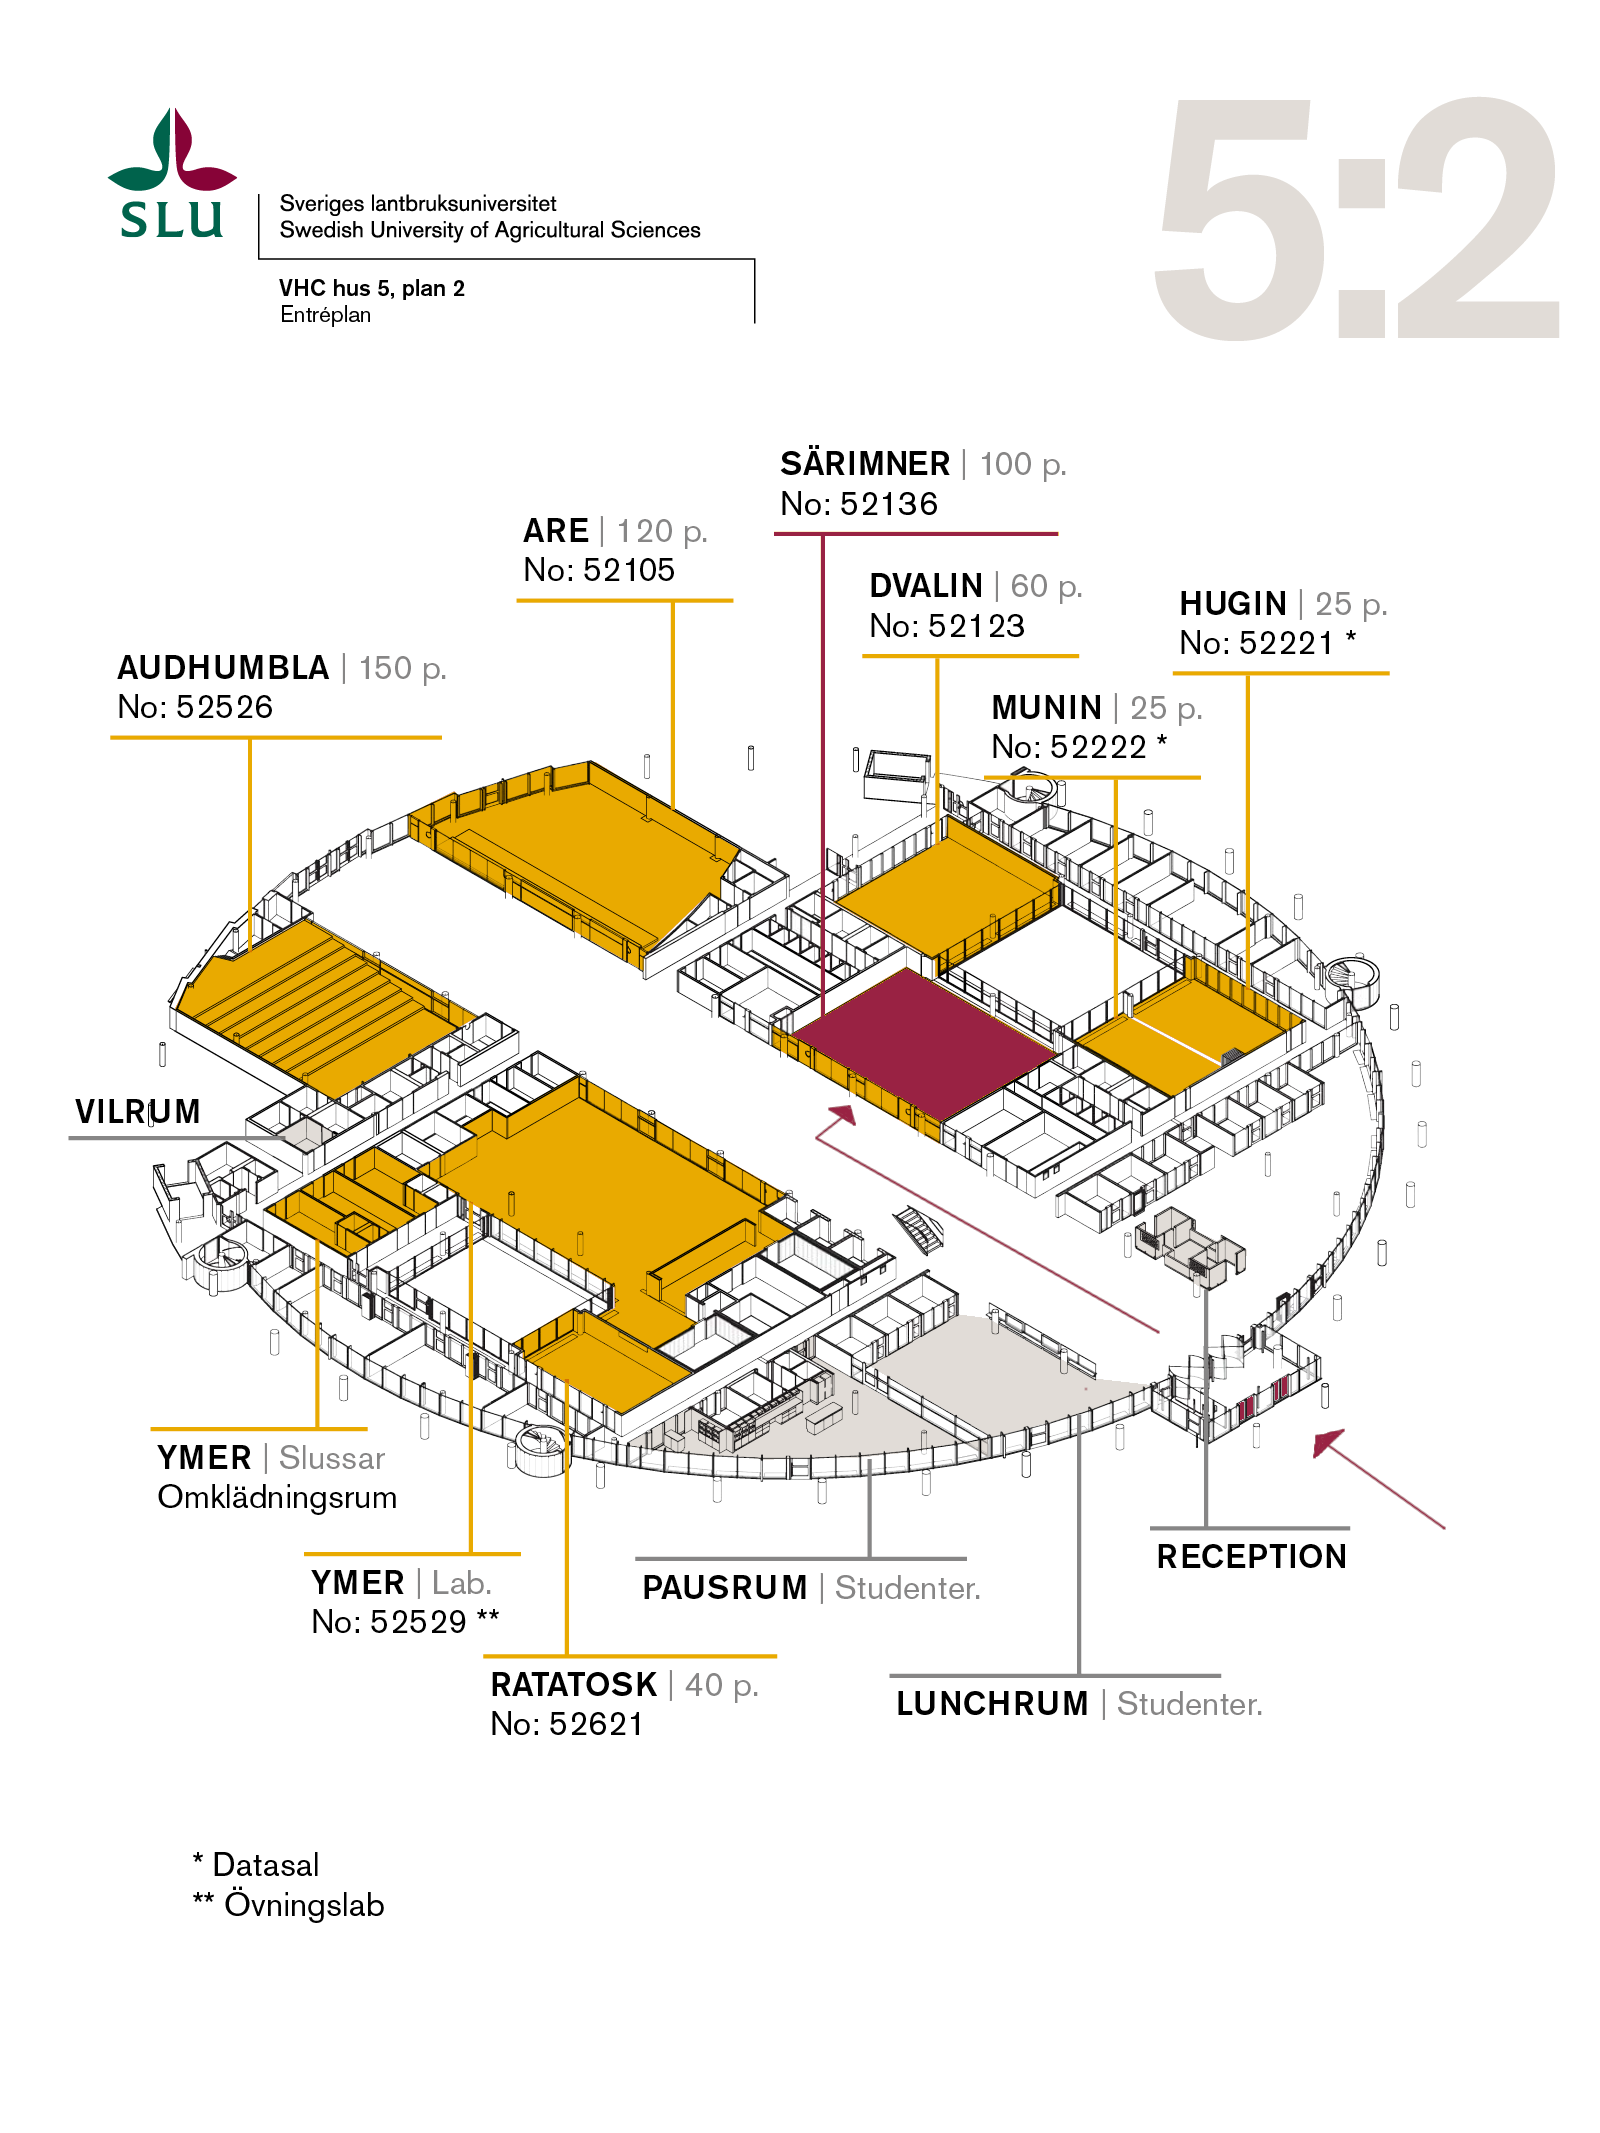
\includegraphics[width=0.8\linewidth]{images/planskiss_vhc_52.png}
\end{center}


\begin{sidewaysfigure}
    \centering
        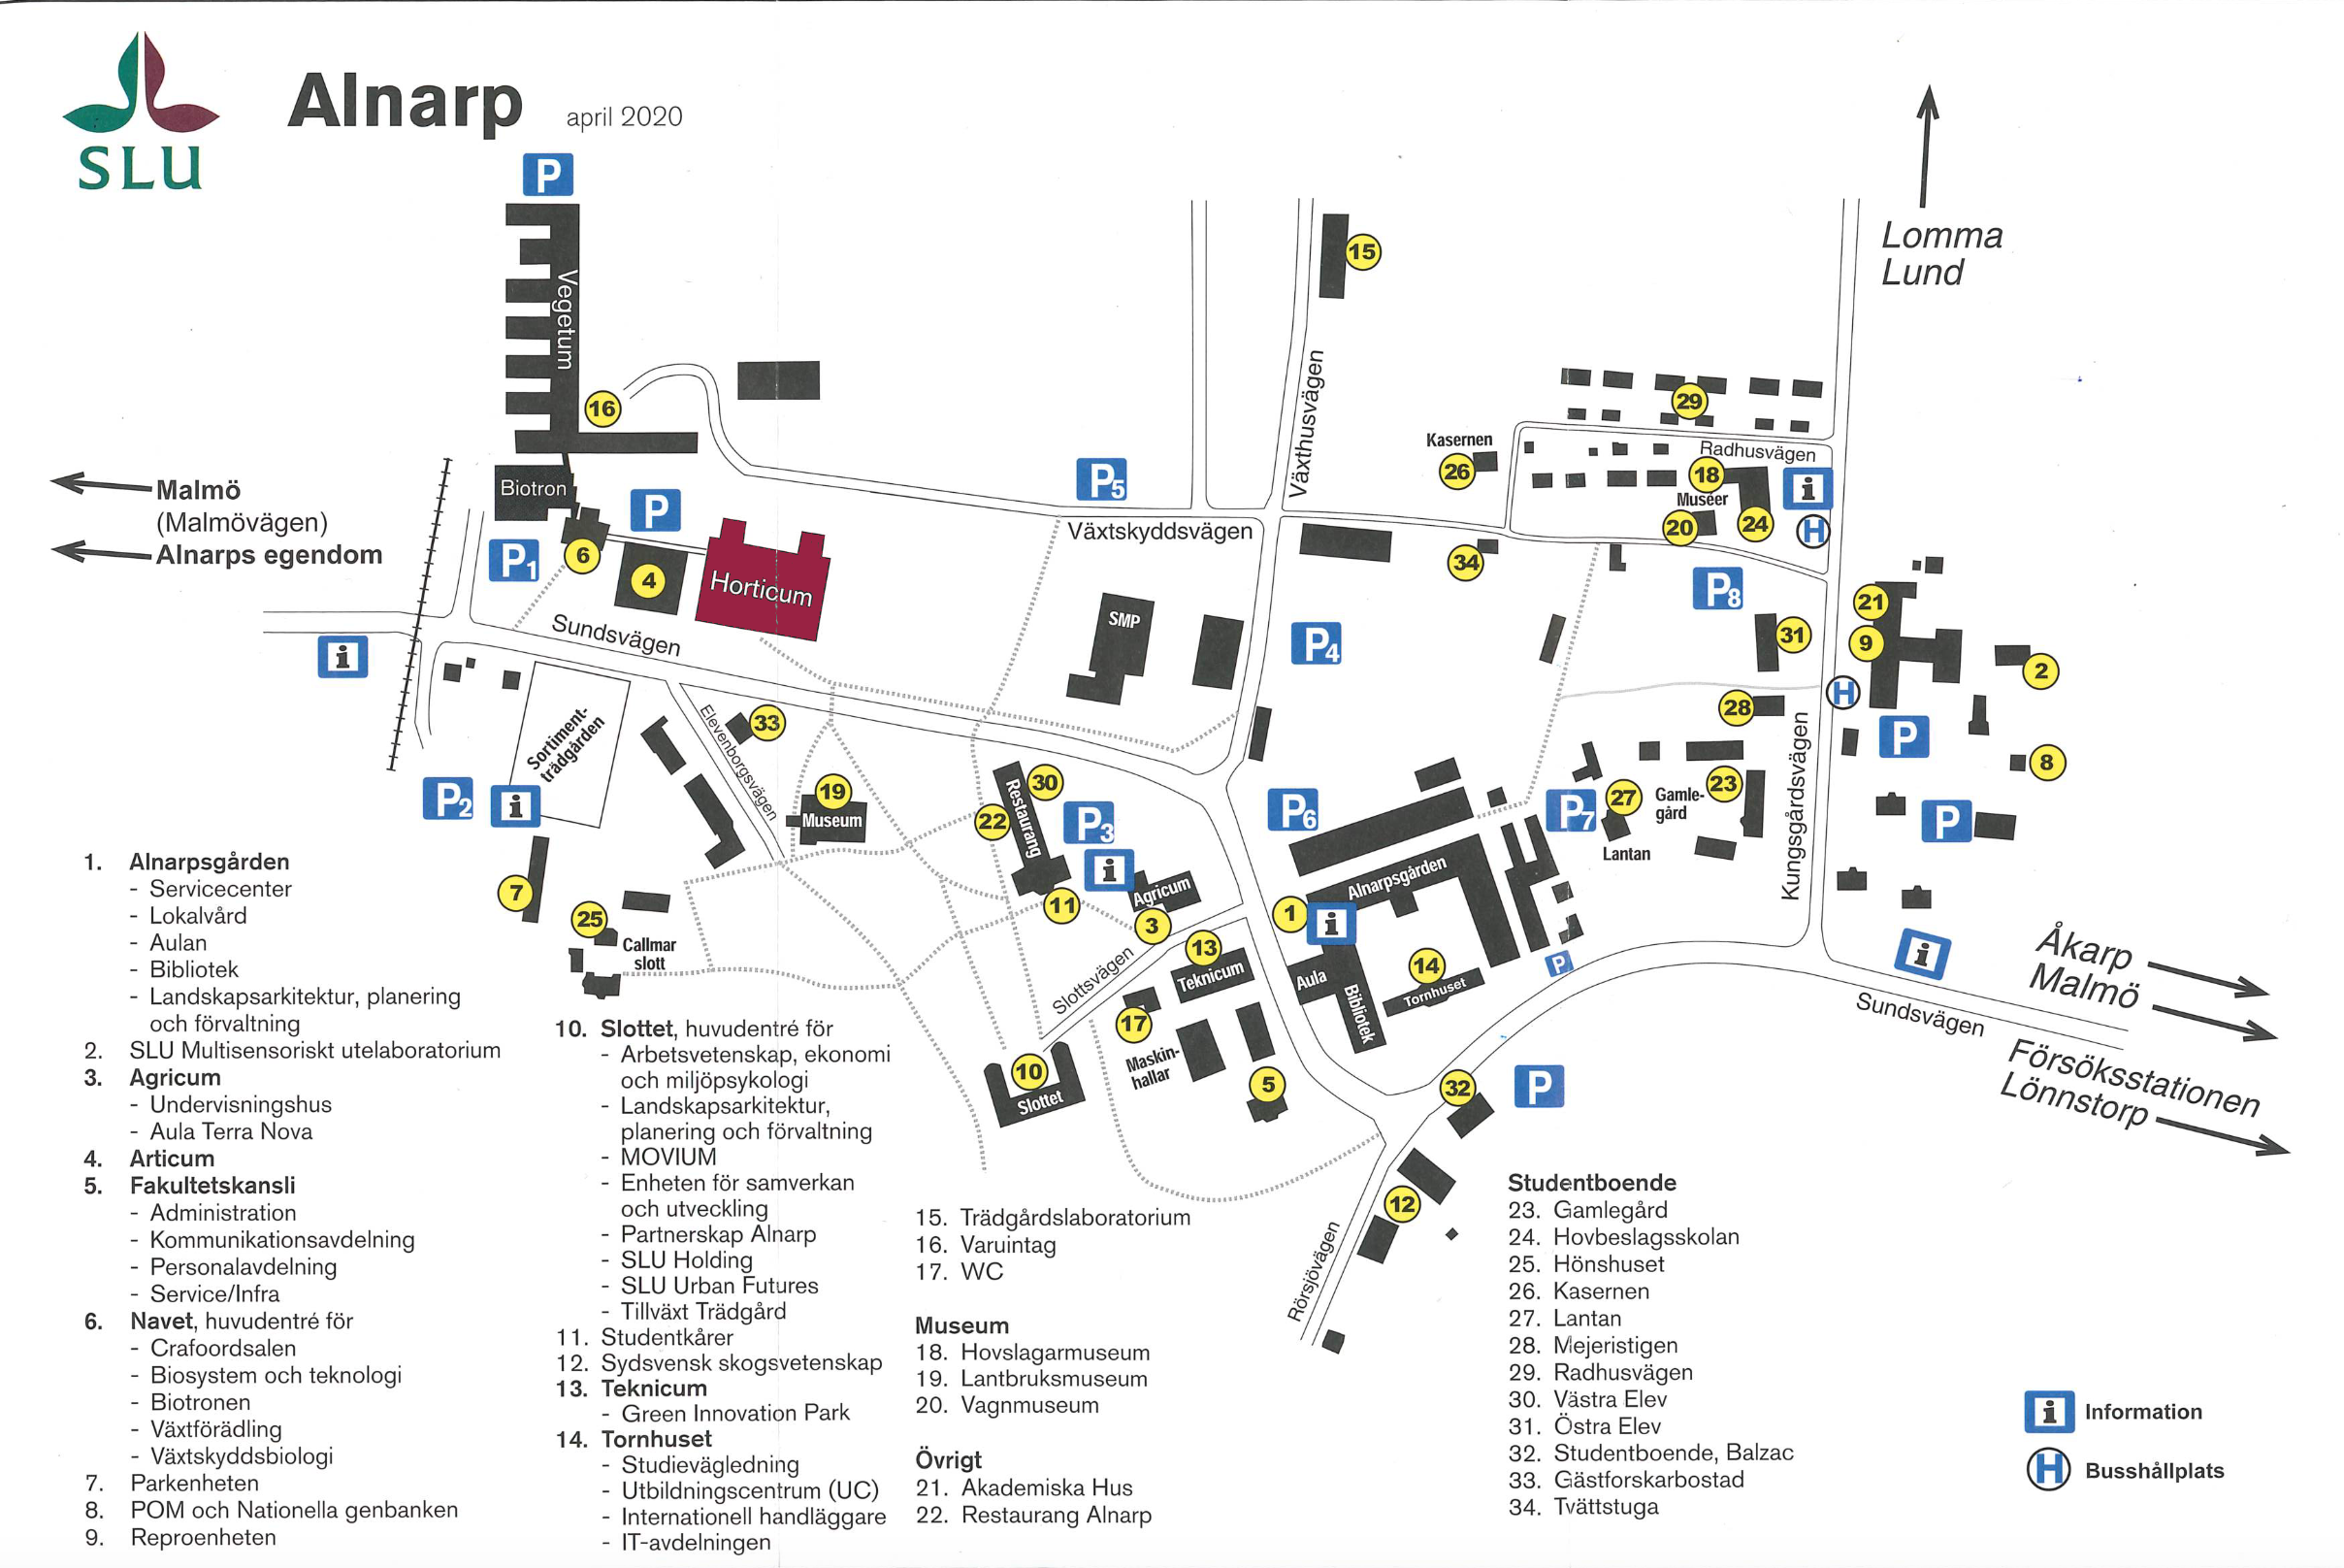
\includegraphics[scale=0.5]{images/CampusAlnarp.png}
\end{sidewaysfigure}

% SPONSORS
%------------------------------------------------------------------
\chapter{Contact Information}

\begin{center}
www.slubi.se

slubi@slu.se
\end{center}

\vfill


\begin{center}

\includegraphics[width=0.5\textwidth]{images/logos/Partnerlogos/slubi.pdf}
\end{center}

\vfill

\newpage

% BACK PAGE
%-----------------------------------------------------------------

\pagecolor{myblue}
\thispagestyle{empty}
\mbox{}

\end{document}
